% Indexes are used to \textbf{speed up} the retrieval of records in response to certain search conditions. The index are stored on disk and provide ways to access the records \textbf{without affecting their physical placement} on the disk. Any field of the file can be used to create an index. A variety of indexes are possible; each of them uses a particular data structure to speed up the search. To find a record or records in the data file based on a search condition on an indexing field, the index is searched, which leads to \textbf{pointers} to one or more disk blocks in the data file where the required records are located. 
\begin{itemize}
    \item An index is an auxiliary file that makes it more efficient to search for records in the data file.
    \item Usually specified on one field of the file, but could be more.
    \item The index file usually occupies considerably less disk blocks than the data file because its entries are much smaller
    \item A binary search on the index yields a pointer to the file record
    \item 
\end{itemize}

\section{Types of Single-Level Ordered Indexes}

An ordered index is similar to an index found at the end of a book. It lists important terms in some defined order (ex: alphabetical) along with the list of pages where the term appears (allows binary search). The alternative (without an index) would be to go page by page in the book to find the requested term (slow !).

For a file with a given record structure consisting of several attributes, an index is defined on a single attribute called \textbf{indexing attribute}.

An index is somewhat similar to dynamic hashing, except that the index search uses the value of the field itself, and not the hashing function's value on that field.

\begin{itemize}
    \item Dense index: there is an index value for each record in the data
    \item Sparse index: there is an index value for some record in the data
\end{itemize}


\begin{table}[]
    \centering
        \begin{tabular}{c|p{5cm}|p{5cm}}
            & Index Field Used for Physical Ordering of the File & Index Field Not Used for Physical Ordering of the File\\\hline
            Indexing field is key & Primary index & Secondary index (Key) \\
            Indexing field is non key & Clustering index & Secondary index (Non Key)\\
        \end{tabular}
    \caption{Comparison of indexes}
    \label{tab:indexesCMP1}
\end{table}


\begin{table}[]
    \centering
        \begin{tabular}{c|p{3cm}|p{3cm}|p{3cm}}
            Type & \# entries & Dense or Nondense(sparse) & Block anchoring on the data file\\\hline
            Primary & \# blocks in data file & Nondense & Yes\\
            Clustering & \# distinct index field values & Nondense & Yes/No\\
            Secondary(key) & \# records in data file & Dense & No\\
            Secondary (nonKey) & \# records or \# distinct field values & Dense or NonDense & No
        \end{tabular}
    \caption{Comparison of indexes}
    \label{tab:indexesCMP2}
\end{table}




\subsection{Primary Indexes}
Ordered file whose records are $<$ Primary key, Block anchor $>$. 
\begin{itemize}
    \item The file records on disk are \textbf{physically ordered} by the primary key, the primary key is thus an \emph{ordering key field}.
    \item There is one index entry \textbf{for each block} in the data file. 
    \item Each index entry has the value of the primary key field for the \textbf{first} record in a block.
    \item The first record of the data file is called the \textbf{anchor record} of the block, or \textbf{block anchor}
\end{itemize}

\paragraph{Insertion and deletion of records}
When inserting a record, we must:
    \begin{enumerate}
        \item Move records to make space for it
        \item Update the index of some entries, because moving records changes anchor records of some blocks
    \end{enumerate}
Reduce the problem by using an unordered overflow file, or a linked list of overflow records for each block in the data file.    

Note that only one primary index may exist, since you can't physically order the data in two different ways.

\subsection{Clustering Indexes}
If the file is physically ordered on a non-key field, that field is called \textbf{clustering field}. A clustering index is also an ordered file whose records are $<$ Clustering field, Disk block pointer$>$.
\begin{itemize}
    \item The file records on disk are physically ordered on the clustering field
    \item There is one entry for each \emph{distinct} value of the clustering field
    \item Each entry contains a pointer to the \emph{first block} in the data that has a record with that value for its clustering field
\end{itemize}
Note that only one clustering index may exist, since you can't physically order the data in two different ways.

One file may only have one clustering index OR one primary index, but not both. 

We could use block anchoring if every distinct value of the ordering field starts a new block.

\paragraph{Insertion and deletion of records}
Still poses problems because the data records are physically ordered. Reduce the problem by reserving a whole block (or a cluster of contiguous blocks) for each value of the clustering field.


\subsection{Secondary Indexes}
A data file can have several secondary indexes in addition to a clustering or primary index.

The field of the index record may be a \emph{non-ordering} \textbf{unique} value or a \textbf{duplicate} value in the data records.
The index is an ordered file whose records are $<$Field, block$|$record pointer$>$. We can't use block anchors, because the data file is not physically ordered by values of the field. 
There are 2 cases:
\begin{itemize}
    \item The field is \textbf{unique}
    \begin{itemize}
        \item One entry per record
        \item Dense index
    \end{itemize}
    \item The field is \textbf{not unique}: Numerous records in the data file can have the same value for the indexing field. Options to implement such an index are:
    \begin{enumerate}
        \item Include \textbf{duplicate} index entries with the same block or record pointer. One entry per record, thus dense index. (binary search must be adapted)
        \item Keep a \textbf{list} of block/record pointers for each value. (binary search must be adapted)
        \item Have a \textbf{single entry} for each \emph{index field value}, but create an extra level of \textbf{indirection} to handle the multiple pointers. For an index entry $<$K,P$>$, the block pointer $P$ points to a block of record pointers (a set of them), which point to records with value $K$. Binary search must not be changed and insertion of new records is straightforward. This is the option generally used.
    \end{enumerate}


\section{Multi-Level indexes}
In a single ordered index file, we use binary search to divide the search space in half. The idea with multilevel indexes is to divide it in $n (=$ the fan-out) at each step. Values for the fan-out are in the order of $300$.
See figure \ref{fig:chap17-multilevel} for an example.
\begin{figure}
    \centering
    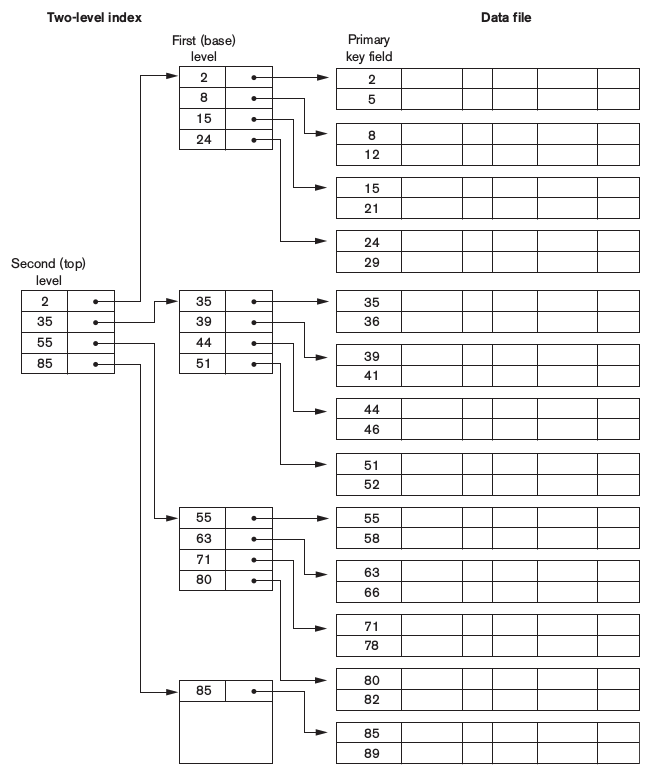
\includegraphics[scale=0.3]{chap17-1}
    \caption{A two-level primary index}
    \label{fig:chap17-multilevel}
\end{figure}

\paragraph{Insertion and deletion} use B-tree or B+-tree data structures. A node corresponds to a disk block, each node is kept between half full and completely full. We must keep the tree balanced on insertion and deletion.

\begin{itemize}
    \item Insertion
    \begin{itemize}
        \item Into a node that is not full is quite efficient
        \item If a node is full the insertion causes a split into
two nodes
        \item Splitting may propagate to other tree levels
    \end{itemize}
    \item Deletion
    \begin{itemize}
        \item Quite efficient if a node does not become less
than half full
        \item If causes a node to become less than half full,
it must be merged with neighboring nodes
    \end{itemize}
\end{itemize}

\begin{itemize}
    \item In a B-tree, pointers to data records exist
at all levels of the tree
    \item In a B+-tree, all pointers to data records
exists at the leaf-level nodes
    \item A B+-tree can have less levels (or higher
capacity of search values) than the
corresponding B-tree
\end{itemize}

Big chapter on B-tree etc... See book because not important.

\end{itemize}